\chapter{Grundlagen und Begriffe}


\begin{mydef}[Graph]Ein Graph $G$ ist ein 2-Tupel $G=(V,E)$. Dabei ist
 $V$ eine endliche Menge von Knoten und
 $E \subseteq \{\{u,v\} \ |\ u,v \in V \wedge u \neq v\}$ die Menge an Kanten.

Eine Kante $\{u,v\}$ wird abgekürzt durch $uv$.
\end{mydef}

\begin{mydef}[Hypergraph]
Ein Hypergraph $H$ ist ein 2-Tupel $H=(V,\mathcal{E})$.  Dabei ist
 $V$ eine endliche Menge von Knoten und
 $\mathcal{E} \subseteq \{e \ |\ e \subseteq V \wedge e \neq \emptyset\}$ die Menge an Kanten.
\end{mydef}

\begin{mydef}[Teilgraph]
Es sei $T=(V_t,E_t)$ ein Graph. $T$ ist Teilgraph des Graphen $G=(V,E)$ genau
dann, wenn $V_t \subseteq V$ und $e \in E_t \Rightarrow e \in E$.
Gilt für alle $u,v \in V_t$ zusätzlich $uv \in E \Rightarrow uv \in E_t$, dann
ist $T$ ein \emph{induzierter} Teilgraph.

Falls $T$ ein induzierter Teilgraph von $G$ ist, so wird $T$ auch als $G[V_t]$ bezeichnet.
\end{mydef}

\begin{mydef}[Komplementärgraph]
Sei $G=(V,E)$ ein Graph. Der Graph $\overline{G}=(V,\overline{E})$ wird 
als Komplementärgraph von $G$ bezeichnet. Dabei sei $\overline{E}:=\{uv\ |\ u \neq y \wedge uv \notin E\}$.
\end{mydef}

\begin{mydef}[Nachbarschaft eines Knotens]
Gegeben sei ein Graph $G=(V,E)$. Dann sei $N(v):=\{u\ |\ uv \in E\}$ die \emph{offene} Nachbarschaft des Knotens $v$. Zusätzlich sei $N[v]:=N(v) \cup \{v\}$ die \emph{abgeschlossene} Nachbarschaft von $v$.
\end{mydef}

\begin{mydef}[Nachbarschaft einer Kante]
Gegeben sei ein Graph $G=(V,E)$. Dann seien $N(uv):=(N(u) \cup N(v)) \backslash \{u,v\}$ und $N[uv]:=N(u) \cup N(v)$ die offene und abgeschlossene Nachbarschaft der Kante~$uv$.
\end{mydef}

\begin{mydef}[Zwillinge]
In einem Graphen werden zwei Knoten $u$ und $v$ ($u\neq v$) als Zwillinge bezeichnet (engl. true twins), wenn $N[u]=N[v]$.
\end{mydef}

Bei Zwillingen gilt es zu beachten, dass es sich um eine abgeschlossene Nachbarschaft handelt. Somit müssen zwei Knoten $u$ und $v$ nicht nur die selben Nachbarn haben, sondern auch selbst benachbart sein. Es muss also eine Kante $uv$ vorhanden sein.


\section{Spezielle Graphen}
\begin{mydef}[Pfad, $P_k$]Ein Pfad (engl. chordless path) der Länge $k$ ist ein Graph mit $k$ Knoten $v_1, \ldots, v_k$ und den Kanten $v_iv_{i+1}, 1 \leq i \leq k$.
\end{mydef}

\begin{mydef}[Kreis, $C_k$]Ein Kreis (engl. chordless cycle) der Länge $k$ ist ein Graph mit $k$ Knoten $v_1, \ldots, v_k$ und den Kanten $v_iv_{i+1}, 1 \leq i \leq k$ und $v_k,v_1$.

Kreise der Länge $k\geq 5$ werden auch als \emph{hole} bezeichnet.
\end{mydef}

\begin{mydef}[Clique, $K_i$]Ein Graph $G=(V,E)$ ist eine Clique der Größe~$i$ 
genau dann, wenn $|V|=i$ und $E=\{uv \ |\ u,v \in V \wedge u \neq v\}$.
\end{mydef}

\begin{figure}[htb]
\centering
\hspace*{\fill}
\subfloat[Ein Pfad der Länge 4 ($P_4$)]{\begin{tikzpicture}
  [thick,node distance=.5cm]

  \node[nN] (a) at (-1.125,0) {};
  \node[nN] (b) [right=of a] {};
  \node[nN] (c) [right=of b] {};
  \node[nN] (d) [right=of c] {};
    
 \foreach \x/\y in {a/b,b/c,c/d} {
     \draw (\x) -- (\y);
 }
  
 \foreach \x in {45,135,-45,-135} {
     \node at (\x:1.1cm) {};
 }
\end{tikzpicture}}
\hspace*{\fill}
\subfloat[Ein Kreis der Länge 5 ($C_5$)]{\begin{tikzpicture}
  [thick]

  \foreach \x/\y in {18/a,90/b,162/c,234/d,306/e} {
     \node[nN] (\y) at (\x:0.75cm) {};
  }
 
  \foreach \x/\y in {a/b,b/c,c/d,d/e,e/a} {
      \draw (\x) -- (\y);
  }

  \foreach \x in {45,135,-45,-135} {
     \node at (\x:1.1cm) {};
  }
 
 
  \node[hN] at (-1.125,0) {};
  \node[hN] at (1.25,0) {};
  
\end{tikzpicture}}
\hspace*{\fill}
\subfloat[Eine Clique der Größe 6 ($K_6$)]{\begin{tikzpicture}
  [thick]

  \node[hN] at (-1.125,0) {};
  \node[hN] at (1.25,0) {};
      
 \foreach \x/\y in {0/a,60/b,120/c,180/d,240/e,300/f} {
     \node[nN] (\y) at (\x:0.75cm) {};
 }
 
 \foreach \x/\y in {a/b,a/c,a/d,a/e,a/f,
                 b/c,b/d,b/e,b/f,
                 c/d,c/e,c/f,
                 d/e,d/f,
                 e/f} {
     \draw (\x) -- (\y);
 }

 \foreach \x in {45,135,-45,-135} {
     \node at (\x:1.1cm) {};
 }
  
\end{tikzpicture}}
\hspace*{\fill}
\caption{Die Graphen $P_4$, $C_5$ und $K_6$.}
\label{pic:bsp_PCK}
\end{figure}

\begin{mydef}[Rad-Graph, $W_k$]
Gegeben sein ein $C_k=(V_c,E_c)$. Ein Rad-Graph (engl. wheel graph) $W_k=(V_w,E_w)$ der Größe $k$ sei dann wie folgt definiert:
\begin{align*}
  V_w&:=V_c \cup \{v\} \text{ mit }v \notin V_c \\
  E_w&:=E_c \cup \{uv \ |\ u \in V_c\}
\end{align*}
%\begin{itemize}
%  \item $V_w:=V_c \cup \{v\}$ mit $v \notin V_c$
%  \item $E_w:=E_c \cup \{uv \ |\ u \in V_c\}$
%\end{itemize}
\end{mydef}

\begin{mydef}[Diamond]
Ein Diamond ist ein Graph mit 4~Knoten und 5~Kanten.
\end{mydef}

\begin{mydef}[Gem]
Gegeben sein ein $P_4=(V_p,E_p)$. Der Graph $(V_g,E_g)$ sei dann wie folgt definiert:
\begin{align*}
  V_g&:=V_p \cup \{v\} \text{ mit } v \notin V_p \\
  E_g&:=E_p \cup \{uv \ |\ u \in V_p\}
\end{align*}
Der so erzeugte Graph wird als \emph{Gem} bezeichnet.
\end{mydef}

\floatimage{pic:bsp_WDiaGem}{Die Graphen $W_5$, Diamond und Gem.}{
\hspace*{\fill}
\subfloat[Ein Rad der Größe 5 ($W_5$)]{\begin{tikzpicture}
  [thick,node distance=.5cm]

  \foreach \x/\y in {18/a,90/b,162/c,234/d,306/e} {
     \node[nN] (\y) at (\x:0.75cm) {};
  }
 
  \node[nN] (center) at (0,0) {};
  
  \foreach \x/\y in {a/b,b/c,c/d,d/e,e/a} {
      \draw (\x) -- (\y);
      \draw (\x) -- (center);
  }
  
 \foreach \x in {45,135,-45,-135} {
     \node at (\x:1.1cm) {};
 }
 
  \node[hN] at (-1.125,0) {};
  \node[hN] at (1.25,0) {};

\end{tikzpicture}}
\hspace*{\fill}
\subfloat[Diamond]{\begin{tikzpicture}
  [thick]


  \foreach \x/\y in {0/a,90/b,180/c,-90/d} {
     \node[nN] (\y) at (\x:0.75cm) {};
  }
 
  \foreach \x/\y in {a/b,b/c,c/d,d/a,a/c} {
      \draw (\x) -- (\y);
  }

  \foreach \x in {45,135,-45,-135} {
     \node at (\x:1.1cm) {};
  }
 
 
  \node[hN] at (-1.125,0) {};
  \node[hN] at (1.25,0) {};
  
\end{tikzpicture}}
\hspace*{\fill}
\subfloat[Gem]{\begin{tikzpicture}
  [thick,node distance=.5cm]

  \node[hN] at (-1.125,0) {};
  \node[hN] at (1.25,0) {};

  \node[nN] (a) at (-0.905,0) {};
  \node[nN] (d) at  (0.905,0) {};
  \node[nN] (b) [above right=of a] {};
  \node[nN] (c) [above left=of d] {};
  
  \node[nN] (e) at (-90:0.65cm) {};
        
 %\foreach \x/\y in {0/a,60/b,120/c,180/d,-90/e} {
 %    \node[nN] (\y) at (\x:0.75cm) {};
 %}
 
 \foreach \x/\y in {a/b,b/c,c/d} {
     \draw (\x) -- (\y);
 }

 \foreach \x in {a,b,c,d} {
     \draw (\x) -- (e);
 }

 \foreach \x in {45,135,-45,-135} {
     \node at (\x:1.1cm) {};
 }
  
\end{tikzpicture}}
\hspace*{\fill}
}

\section{Dominating Induced Matchings}
Eine Matching ist eine Teilmenge von Kanten eines Graphen, wobei die Kanten keinen gemeinsamen Knoten besitzen.

\begin{mydef}[Matching]
Gegeben sei ein Graph $G=(V,E)$. Eine Menge $M \subseteq E$ heißt \emph{Matching}, wenn für alle $e,e' \in M$ gilt: $e\cap e' = \emptyset$.
\end{mydef}

Ein dominating induced Matching (dim) zeichnet sich dadurch aus, dass zwischen zwei Kanten des Matchings immer mindestens zwei weitere Kanten liegen, und dass jede Kante, die nicht zum Matching gehört, einen gemeinsamen Knoten mit einer Kante des Matchings besitzt.

\begin{mydef}[dominating induced Matching]
Gegeben sei ein Graph $G=(V,E)$ und ein Matching $M$. $M$ ist ein \emph{dominating induced Matching}, wenn die folgenden Bedingungen erfüllt sind:
\begin{align*}
 %\forall\ e,e' \in M,e\neq e'  &: e\cap e' = \emptyset \wedge \nexists\ xy \in E  \text{ mit } x \in e \wedge y \in e' & \text{\emph{induced}} \\
 \forall\ e,e' \in M&: dist_G(e,e') \geq 2 & \text{\emph{induced}} \\
 \forall\ e \in E \backslash M &: \exists\ e' \in M \text{ mit } e\cap e' \neq \emptyset & \text{\emph{dominating}}
\end{align*}
\end{mydef}

%\begin{mydef}[induced Matching]
%Gegeben sei ein Graph $G=(V,E)$ und ein Matching $M$. $M$ ist ein \emph{induced Matching}, wenn für alle $e,e' \in M$ gilt: $dist_G(e,e') \geq 2$.
%\end{mydef}

%\begin{mydef}[dominating Matching]\label{def:dominatingMatching}
%Gegeben sei ein Graph $G$ und ein Matching $M$. $M$ ist ein \emph{dominating Matching}, wenn für alle $e \in E \backslash M$ gilt: Es existiert ein $e' \in M$ mit $e\cap e' \neq \emptyset$.
%\end{mydef}

Das dazugehörige Entscheidungsproblem (Dominating Induced Matching Problem; kurz~DIM) fragt, ob ein Graph ein solches Matching besitzt. Es wird auch als Efficient Edge Domination Problem (EED) bezeichnet. DIM ist NP-vollständig \cite{dimNPv}.

Das Besondere an DIM ist, dass es sowohl ein Pack- als auch ein Abdeckungsproblem darstellt. Es müssen genug Kanten gewählt werden, damit alle Kanten, die nicht zum Matching gehören mit einer des Matchings verbunden sind. Zwischen den Kanten des Matching müssen sich aber gleichzeitig immer mindestens zwei weitere Kanten befinden.

\todo{Beispiel}
\begin{figure}[htb]
\subfloat[]{\begin{tikzpicture}
  [thick,node distance=.5cm]

  \node[mN] (a) at (-1.125,0) {};
  \node[mN] (b) [right=of a] {};
  \node[nN] (c) [right=of b] {};
  \node[mN] (d) [right=of c] {};
  \node[mN] (e) [right=of d] {};
  \node[nN] (f) [below=of c] {};
    
    \begin{pgfonlayer}{background}
        \foreach \x/\y in {a/b,d/e} {
            \draw [very thick,-,darkgreen] (\x.center) -- (\y.center);
        }

        \foreach \x/\y in {b/c,c/d} {
            \draw [very thick,-,blue] (\x.center) -- (\y.center);
        }
        
        \draw [very thick,-,red] (c.center) -- (f.center);
        
    \end{pgfonlayer}

 \foreach \x/\y in {a/b,b/c,c/d,d/e,c/f} {
     %\draw (\x) -- (\y);
 }
  
\end{tikzpicture}}
\hspace*{\fill}
\subfloat[]{\begin{tikzpicture}
  [thick,node distance=.5cm]

  \node[nN] (a) at (-1.125,0) {};
  \node[nN] (b) [right=of a] {};
  \node[nN] (c) [right=of b] {};
  \node[nN] (d) [right=of c] {};
  \node[nN] (e) [right=of d] {};
  \node[nN] (f) [below=of c] {};
    
    \begin{pgfonlayer}{background}
        \foreach \x/\y in {b/c} {
            \draw [line width=0.075cm,-,darkgreen] (\x.center) -- (\y.center);
        }

        \foreach \x/\y in {a/b,c/d,c/f} {
            \draw [line width=0.075cm,-,orange] (\x.center) -- (\y.center);
        }
        
        \draw [line width=0.075cm,-,violet] (d.center) -- (e.center);
        
    \end{pgfonlayer}

 \foreach \x/\y in {a/b,b/c,c/d,d/e,c/f} {
     %\draw (\x) -- (\y);
 }
  
\end{tikzpicture}}
\hspace*{\fill}
\subfloat[]{\begin{tikzpicture}
  [thick,
   normalN/.style={circle,draw,minimum size=0.25cm,inner sep=0pt,fill=white},
   node distance=.5cm]

  \node[normalN] (a) at (-1.125,0) {};
  \node[normalN] (b) [right=of a] {};
  \node[normalN] (c) [right=of b] {};
  \node[normalN] (d) [right=of c] {};
  \node[normalN] (e) [right=of d] {};
  \node[normalN] (f) [below=of c] {};

    
    \begin{pgfonlayer}{background}
        \foreach \x/\y in {a/b,d/e} {
            \draw [line width=0.075cm,-,bgred] (\x.center) -- (\y.center);
        }

        \foreach \x/\y in {b/c,c/d} {
            \draw [line width=0.075cm,-,bgblue] (\x.center) -- (\y.center);
        }
        
        \draw [line width=0.075cm,-,darkgreen] (c.center) -- (f.center);
        
    \end{pgfonlayer}

 \foreach \x/\y in {a/b,b/c,c/d,d/e,c/f} {
     %\draw (\x) -- (\y);
 }
\end{tikzpicture}}
\caption{Die Graphen $P_4$, $C_5$ und $K_6$.}
\label{pic:bsp_DIM}
\end{figure}

\begin{figure}[htb]
\centering
\begin{tikzpicture}
  [thick,
   normalN/.style={circle,draw,minimum size=0.25cm,inner sep=0pt,fill=white},
   greenN/.style={normalN,fill=bggreen},
   node distance=.5cm]

  \node[normalN] (a) at (-1.125,0) {};
  \node[normalN] (b) [right=of a] {};
  \node[normalN] (c) [right=of b] {};
  \node[normalN] (d) [right=of c] {};
  \node[normalN] (e) [right=of d] {};
  \node[normalN] (f) [below=of c] {};
  \node[normalN] (g) [below=of f] {};
  
    \begin{pgfonlayer}{background}
        \foreach \x/\y in {a/b,d/e,f/g} {
            \draw [line width=0.075cm,darkgreen] (\x.center) -- (\y.center);
        }

        \foreach \x/\y in {b/c,c/d,c/f} {
            \draw [line width=0.075cm,-,bgblue] (\x.center) -- (\y.center);
        }
    \end{pgfonlayer}

 \foreach \x/\y in {a/b,b/c,c/d,d/e,c/f,f/g} {
     %\draw (\x) -- (\y);
 }
  
\end{tikzpicture}
\caption{TODO}
\label{pic:bsp_BnB_1}
\end{figure}

\subsection{dims in einfachen Klassen von Graphen}
Zwar ist es schwierig für einen beliebigen Graphen zu sagen, ob er ein dim besitzen und welche Kante dazu gehört. Über einige einfachen (Klassen von) Graphen lassen sich jedoch Aussagen treffen.

\subsection{Pflichtkanten}
\todo{Eventuell andere Übersetzung oder engl Begriff}

Für einen Graphen ist ein dim nicht immer eindeutig. Es kann mehrere mögliche Varianten in einem Graphen geben. Es ist jedoch so, dass in einigen Fällen auch bei verschiedenen dims, einzelne Kanten zwingend in jedem dim des Graphen enthalten sein müssen.

\begin{mydef}[Pflichtkante]
Gegeben sei ein Graph $G=(V,E)$. Eine Kante $m\in E$ ist eine \emph{Pflichtkante} (engl.: mandatory edge), wenn für alle dims $M$ von $G$ gilt: $m\in M$.
\end{mydef}

In einem Diamond $D$ ist beispielsweise die mittlere Kante eine Pflichtkante. Wählt man eine andere Kante (am Rand), so ist die gegenüberliegende Kante zu nahe an der gewählten um zum dim zu gehören. Wenn $D$ Teilgraph eines größeren Graphen ist, bliebe noch die Möglichkeit, dass die gegenüberliegende Kante mit einer Kante das dims verbunden ist. Auch das ist nicht möglich, da diese Kanten ebenfalls zu nahe wären.

\todo{alternativ über Knotenklassen beschrieben, oder vorher zeigen, dass in einem Dreieck eine Katenenthalten sein muss.}

\begin{figure}[htb]
\centering
\hspace*{\fill}
\subfloat[Diamond]{\begin{tikzpicture}
  [thick,
   normalN/.style={circle,draw,minimum size=0.25cm,inner sep=0pt,fill=white},
   colE/.style={draw,-,line width=0.075cm}
  ]

  \foreach \x/\y in {0/a,90/b,180/c,-90/d} {
     \node[normalN] (\y) at (\x:0.75cm) {};
  }

  \node (e) at (0:1.5cm) {};
  
    \begin{pgfonlayer}{background}
        \draw [colE,blue] (c.center) -- (b.center);
        
        \draw [colE,darkgreen] (a.center) -- (b.center);
        \draw [colE,darkgreen] (a.center) -- (c.center);
        \draw [colE,darkgreen] (c.center) -- (d.center);
        
        \draw [colE,red] (a.center) -- (d.center);

        \draw [colE,red, dashed] (a.center) -- (e.center);
    \end{pgfonlayer}
   
 
\end{tikzpicture}}
\hspace*{\fill}
\subfloat[Gem]{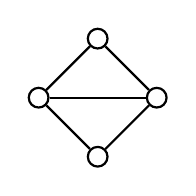
\begin{tikzpicture}
  [thick,
   normalN/.style={circle,draw,minimum size=0.25cm,inner sep=0pt,fill=white}
  ]

  \foreach \x/\y in {0/a,90/b,180/c,-90/d} {
     \node[normalN] (\y) at (\x:0.75cm) {};
  }
  
  \foreach \x/\y in {a/b,b/c,c/d,d/a,a/c} {
      \draw (\x) -- (\y);
  }

 
\end{tikzpicture}}
\hspace*{\fill}
\caption{TODO}
\label{pic:bsp_mandEdge}
\end{figure}

\section{Cographen}

\begin{mydef}[Join zweier Graphen]
Gegeben seien die Graphen $G_1=(V_1,E_1)$ und $G_2=(V_2,E_2)$ mit $V_1 \cap V_2=\emptyset$. Der Graph $G_j=(V_j,E_j)$ sei dann wie folgt definiert:
\begin{align*}
V_j&:=V_1\cup V_2 \\
E_j&:=E_1\cup E_2 \cup \{uv\ |\ u\in V_1,v\in V_2\}
\end{align*}
$G_j=G_1\join G_2$ wird als \emph{Join} von $G_1$ und $G_2$ bezeichnet.
\end{mydef}

\begin{mydef}[Cojoin zweier Graphen]
Gegeben seien die Graphen $G_1=(V_1,E_1)$ und $G_2=(V_2,E_2)$ mit $V_1 \cap V_2=\emptyset$. Der Graph $G_c=(V_c,E_c)$ sei dann wie folgt definiert:
\begin{align*}
V_j&:=V_1\cup V_2 \\
E_j&:=E_1\cup E_2
\end{align*}
$G_c=G_1\cojoin G_2$ wird als \emph{Cojoin} von $G_1$ und $G_2$ bezeichnet.
\end{mydef}

\begin{mydef}[Cograph]
Ein Graph heißt \emph{Cograph}, wenn er aus einzelnen Knoten durch endliche Anwendungen von Join und Cojoin erzeugt werden kann.
\end{mydef}

Cographen sind $P_4$ frei und jeder induzierte Teilgraph eines Cographen ist ebenfalls ein Cograph. \cite{CographsP4free}